%%=============================================================================
%% Methodologie
%%=============================================================================

\chapter{\IfLanguageName{dutch}{Methodologie}{Methodology}}
\label{ch:methodologie}

Binnen dit experiment zullen er concreet 3 specifieke toestanden van een Android apparaat met elkaar vergeleken worden. Het eerste geval is een Android apparaat waarop er nog geen enkele wijziging is doorgevoerd. Deze staat dus nog gelijk met de fabrieksinstellingen van het apparaat. Bij het tweede geval zijn de instellingen zo aangepast om de dataverzameling van Google te minimaliseren. Bij deze toestand wordt er optimaal gebruik gemaakt van de mogelijkheden die Google en het Android besturingssysteem zodat er zo min mogelijk data wordt verzameld. In het derde geval zullen er methodes gebruikt worden, die niet direct door Google of Android zelf worden ondersteund, om zo Google volledig te proberen elimineren van het apparaat.

Bij deze drie gevallen zal er in detail beschreven worden welke stappen precies moeten worden genomen om de testtoestand van het apparaat te bekomen. Daarna zal het internetverkeer van elk geval geanalyseerd worden gedurende 1 uur. Concreet wordt er hier geregistreerd hoeveel keer er gemiddeld data wordt verstuurd naar specifieke internet domeinen van Google.

\section{Testapparaat}
\label{sec:testapparaat}
Het experiment zal plaatsvinden op een Oneplus 5 apparaat (model nr. ONEPLUS A500). Dit apparaat draait op een aangepaste versie van Android, genaamd OxygenOS. OxygenOS is een Android ROM die gekend is voor het toevoegen van configureerbaarheid en handige functies, terwijl de 'look and feel' grotendeels gelijkt blijft in vergelijking met stock Android. De bloatware die hierbinnen wordt meegeleverd is ook minimaal. De laatste versie van OxygenOS die beschikbaar is op het moment van schrijven, is OxygenOS 9.0.5, die verderbouwt op Android 9.0, ofwel Android Pie.

\section{Testgevallen}
\label{sec:testgevallen}

In deze sectie zullen de verschillende testgevallen in detail besproken worden.

\subsection{Testgeval 1: Android met fabrieksinstellingen}
\label{sec:testgeval1}
Binnen dit geval zal gebruik gemaakt worden van een Android apparaat waarbij buiten de initiële setup geen wijzigingen zijn gebeurd. Om in deze toestand terecht te raken zal er binnen OxygenOS gebruik worden gemaakt van de functie 'Alle gegevens wissen (fabrieksinstellingen terugzetten)'. Dit is te vinden in de 'Instellingen' applicatie, onder 'Systeem' >  'Opties voor resetten' > 'Alle gegevens wissen (fabrieksinstellingen terugzetten)'. Wanneer er naar het juiste scherm genavigeerd is, wordt er ook gekozen om de interne opslag te wissen, zoals te zien in figuur \ref{fig:fabrieksinstellingen}.

\begin{figure}
    \centering
    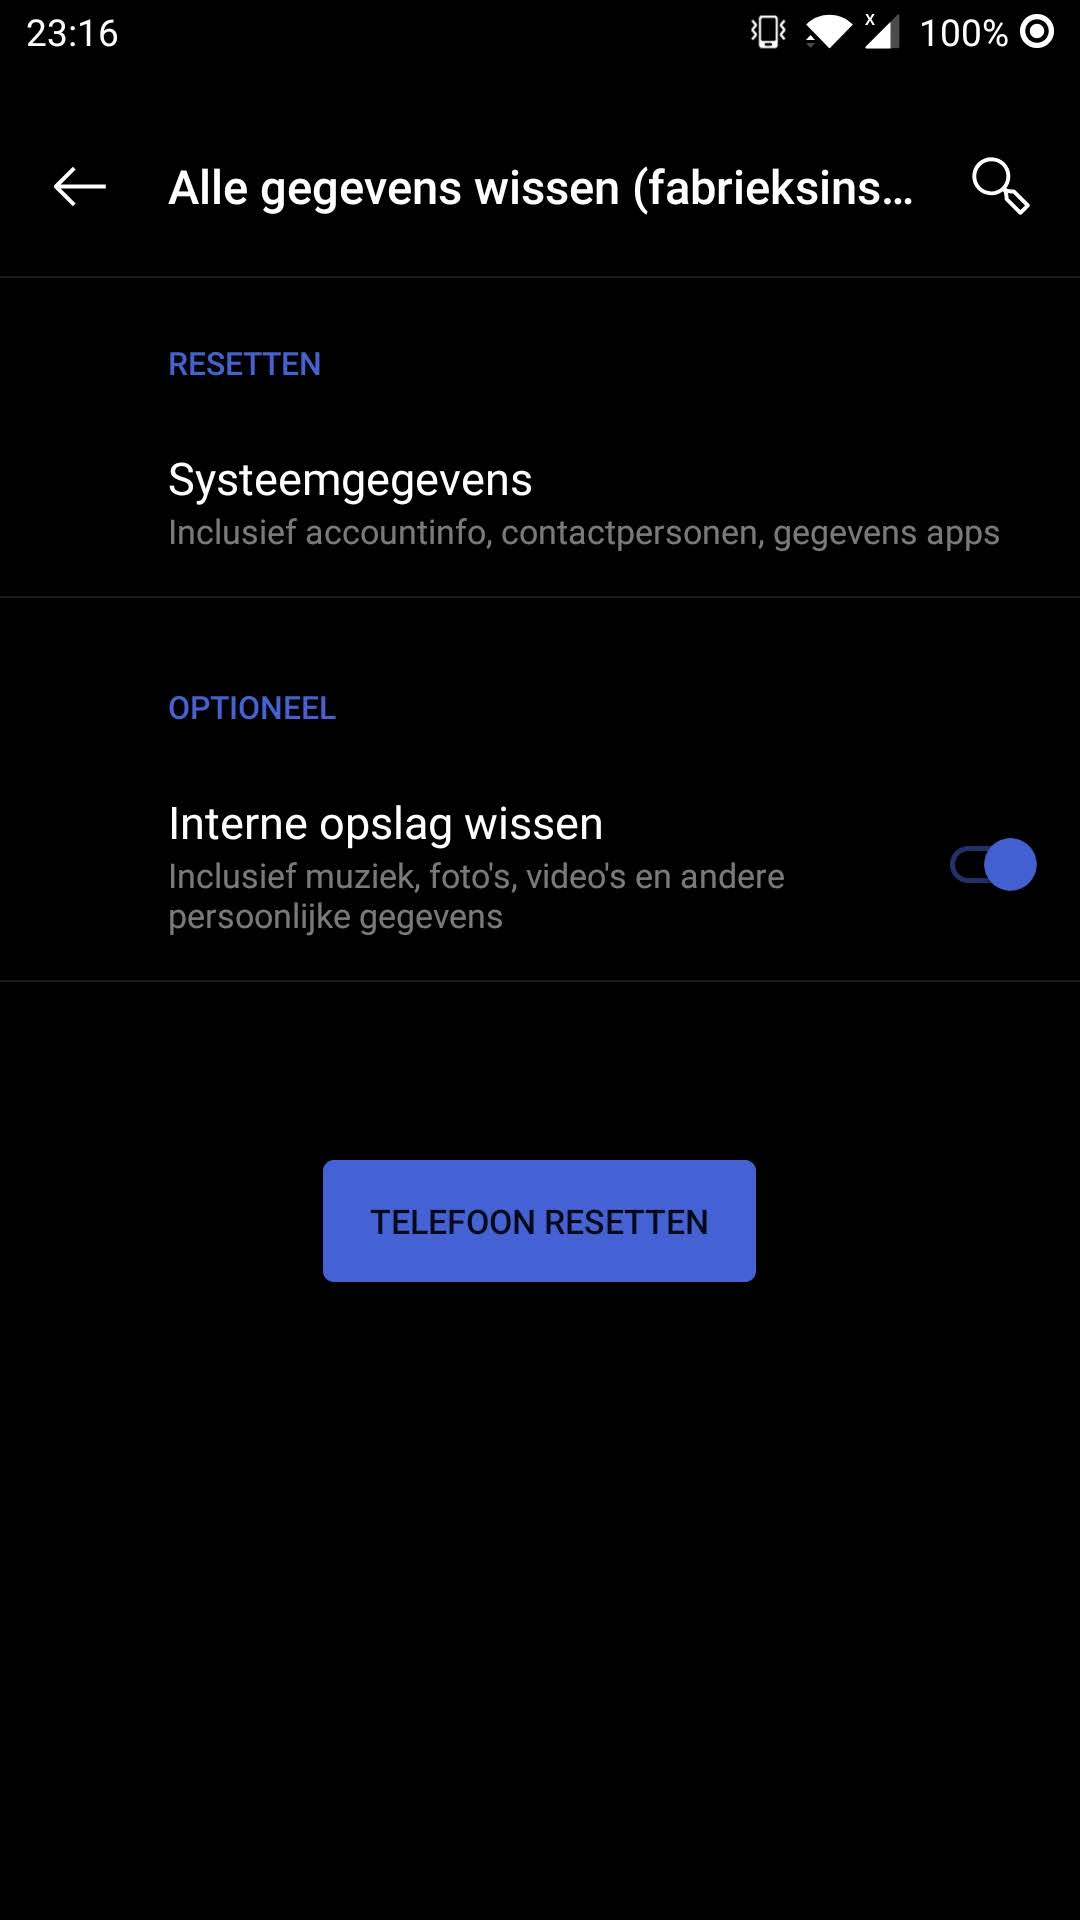
\includegraphics[width=0.4\textwidth]{img/fabrieksinstellingen.jpg}
    \caption{Screenshot van het scherm waar alle gegevens gewist kunnen worden en de fabrieksinstellingen kunnen worden teruggezet}
    \label{fig:fabrieksinstellingen}
\end{figure}


\subsection{Testgeval 2: Android met aangepaste instellingen}
\label{sec:testgeval2}
Binnen dit geval zal gebruik gemaakt worden van een Android apparaat waarbij de instellingen zo zijn aangepast zodat de verzameling van data geminimaliseerd wordt. Dit zal gedaan worden via de 'zachte' methoden die besproken werden in het literatuuronderzoek (\ref{softmethods}).

\subsection{Testgeval 3: Aangepaste versie van Android}
\label{sec:testgeval3}
Binnen dit geval zal gebruikt gemaakt worden van een Android apparaat waarop LineageOS op geïnstalleerd. LineageOS is een custom ROM (zie \ref{installcustomrom}) waarbij Google Apps niet is inbegrepen in het besturingssysteem. Er zal gebruik gemaakt worden van de laatste officiële versie van LineageOS voor dit apparaat, namelijk 16.0, die te vinden is op \url{https://download.lineageos.org/cheeseburger} (de term 'cheeseburger' in de URL is de codenaam voor de 'Oneplus 5', het testapparaat).

\section{Software voor monitoring netwerkactiviteit}
\label{sec:metingsoftware}
Het verzamelen van data die de netwerkactiviteit van het apparaat beschrijft, zal op een gelijkaardige manier worden gedaan zoals in het onderzoek door \cite{schmidt_google-data-collection}, wat ook in de litatuurstudie werd besproken. Om exact te kunnen zien welke data er precies binnenkomt en buitengaat via het internet op het apparaat, is er extra software nodig. Deze optie wordt namelijk niet gegeven door het Android besturingssysteem zelf. De software die wij gebruiken moet voldoen aan enkele voorwaarden:
\begin{itemize}
    \item De verkregen data moet kunnen worden geëxporteerd naar een bruikbaar formaat.
    \item De software mag geen aanpassing maken aan of vereisen van het apparaat.
    \item De software moet de gevraagde data verzamelen zonder dat deze wordt beïnvloed door de software zelf.
\end{itemize}
Er bestaan reeds veel applicaties die rechstreeks vanaf het Android apparaat deze data kan verzamelen. Velen hiervan vallen al direct weg, aangezien ze root toegang vereisen. De 'geroote' toestand is namelijk een voorwaarde van de testgevallen, waardoor we deze doorheen de gevallen niet ingeschakeld kunnen houden. 

De uiteindelijke gekozen software is 'Charles Proxy'. De techniek die hierbij wordt gehanteerd heet 'MITM proxy', wat letterlijk 'Man-In-The-Middle proxy' betekent. Zoals de naam al zegt is dit een proxy die als 'tussenman' tussen het apparaat en het internet zal staan, en zo alle netwerkactiveit zal kunnen monitoren. Wanneer deze applicatie draait op een computer binnen een netwerk, moeten er op het Android apparaat nog 2 extra instellingen gebeuren voordat al het netwerkverkeer kan worden opgevolgd. Eerst en vooral moet het Android apparaat verbonden zijn met hetzelfde netwerk als de computer waarop Charles draait. Daarna moet er gekeken worden wat het lokale IP-adres is van deze computer binnen het netwerk. Op windows computers kan deze gevonden worden via het 'ipconfig' commando en op Mac computers via het 'ifconfig' commando. Eens gevonden moet dit IP-adres als proxy ingevoerd worden in de netwerkinstellingen binnen het Android apparaat. Dit kan gedaan worden door te navigeren naar de Wi-Fi instellingen, het verbonden netwerk te selecteren en dan op het potloodje te drukken om de instellingen van dit netwerk te wijzigen. Bij 'Hostnaam van proxy' moet dan het lokaal IP-adres van de computer worden ingegeven, en in het 'Proxy-Poort' veld 8888 (Dit is de standaard poort die Charles Proxy gebruikt). Vanaf nu zal al het netwerkverkeer door deze proxy getunnelt worden, maar als er naar een site wordt gesurft op het Android apparaat zal er nog steeds een melding worden weergegeven die zegt dat er geen internetverbinding is. Dit komt door 2 redenen.

\begin{itemize}
    \item De Charles applicatie heeft het Android apparaat nog geen toegang gegeven
    \item Charles gebruikt zijn eigen SSL certificaat, dat nog niet als een vertrouwd certificaat wordt beschouwd binnen het Android apparaat.
\end{itemize}

Zodra het Android apparaat een verbinding probeert te maken met een website zal Charles een melding tonen die vraagt of het apparaat dat probeert verbinding te maken wel degelijk toegang mag hebben tot de proxy, zoals te zien in figuur \ref{fig:charlesmelding}. Hier dient op 'allow' geklikt te worden. 

\begin{figure}
    \centering
    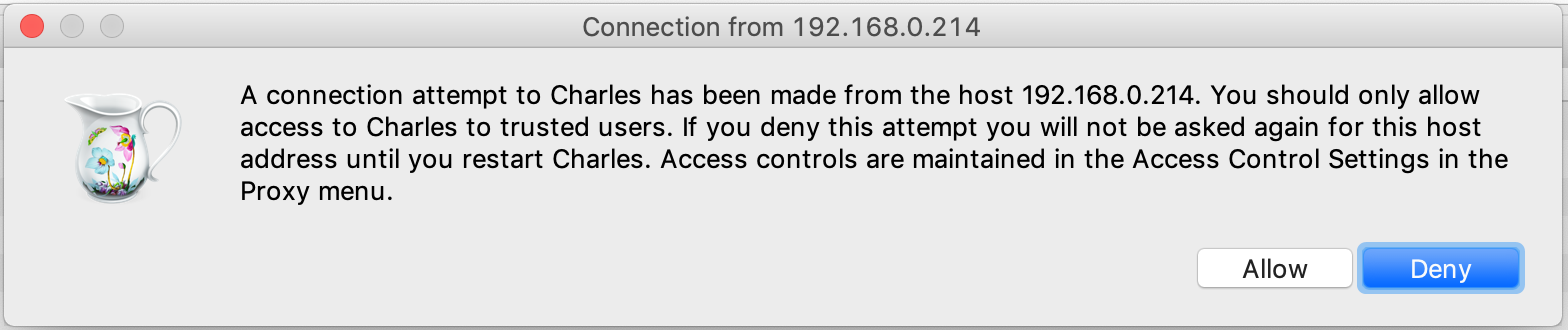
\includegraphics[width=1\textwidth]{img/charlesmelding.png}
    \caption{Screenshot van de melding die Charles geeft wanneer er een nieuwe onbekende verbinding binnenkomt}
    \label{fig:charlesmelding}
\end{figure}

Vanaf dit moment kan het Android apparaat theorethisch gezien verbinden met het internet, doorheen de proxy. Applicaties zullen dit echter niet toestaan, omdat het SSL certificaat dat Charles gebruikt niet gekend is (figuur \ref{fig:charlescantconnect}). Door op het apparaat naar \url{http://www.charlesproxy.com/getssl/} (de enige pagina die browser wel zal kunnen bereiken) te surfen, wordt het Charles certificaat gedownload, en kan deze geïnstalleerd worden op het apparaat, zoals te zien in figuur \ref{fig:charlessslcertificateinstall}.

\begin{figure}
    \centering
    \begin{subfigure}{.5\textwidth}
        \centering
        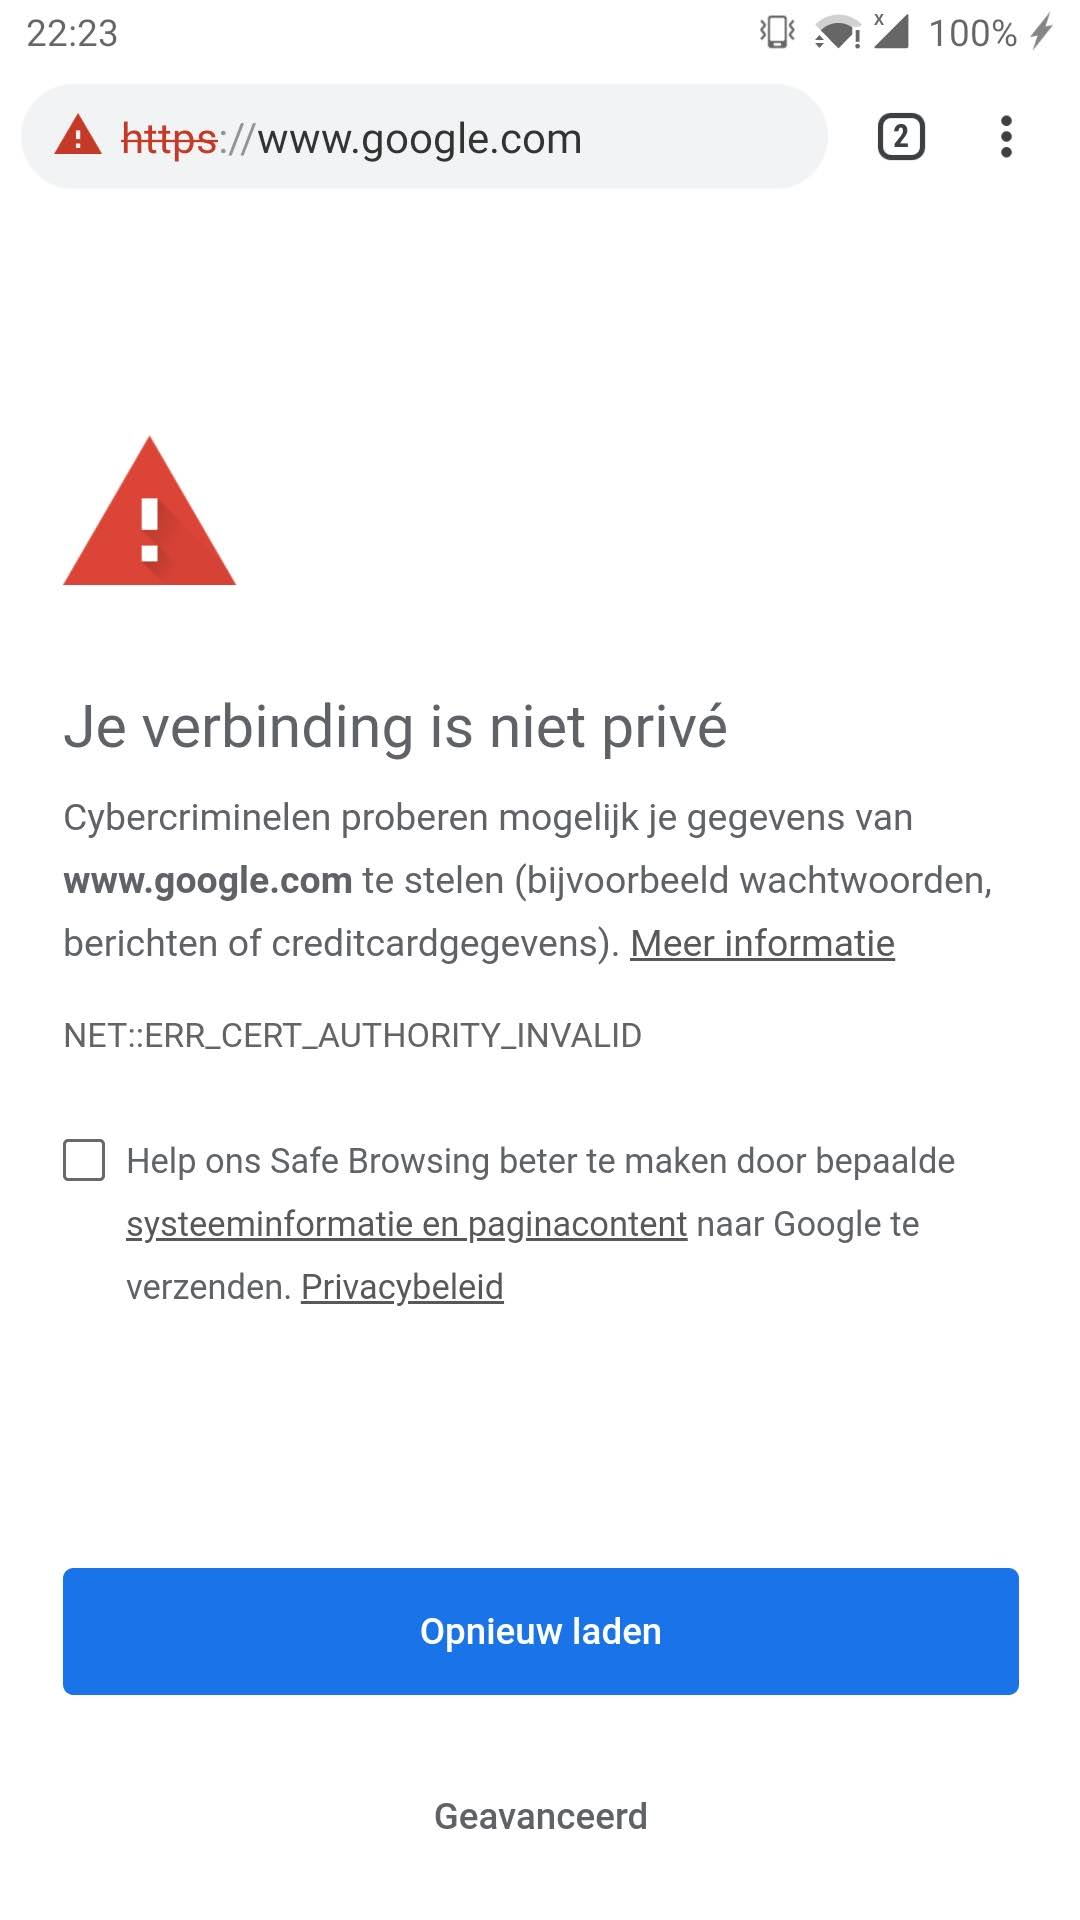
\includegraphics[width=0.8\linewidth]{img/charlescantconnect.jpg}
        \caption{Sites kunnen niet bereikt worden door een onveilig certificaat}
        \label{fig:charlescantconnect}
    \end{subfigure}%
    \begin{subfigure}{.5\textwidth}
        \centering
        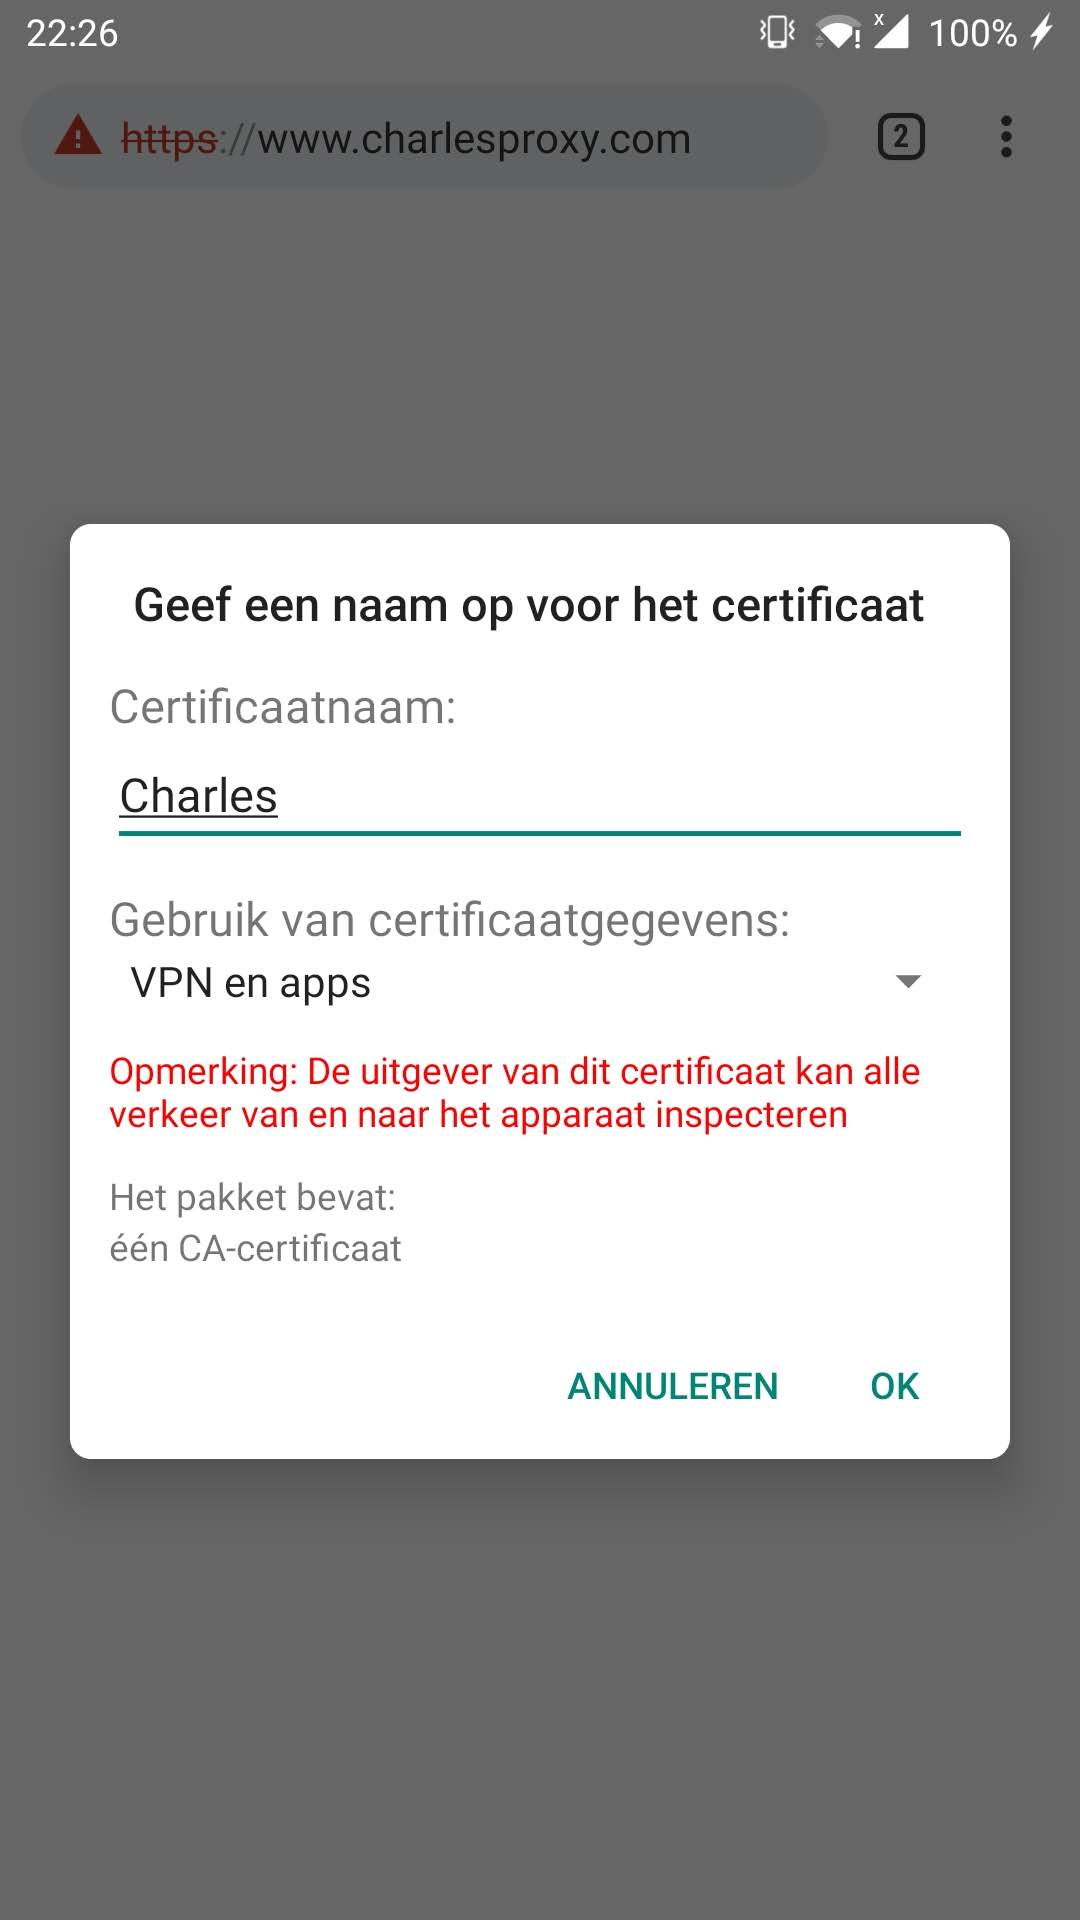
\includegraphics[width=0.8\linewidth]{img/charlessslcertificateinstall.jpg}
        \caption{Installatie van het gedownloade Charles SSL certificaat}
        \label{fig:charlessslcertificateinstall}
    \end{subfigure}
    \caption{Het Charles SSL certificaat downloaden en gebruiken}
\end{figure}

In de 'SSL Proxying Settings' moet ingesteld worden dat SSL  verzoeken naar alle domeinen door de proxy gehaald worden, zodat ook hiervan de inhoud in vlakke tekst kan bekeken worden. Deze instelling is te zien in figuur \ref{fig:charlessslsettings} door middel van de locatie '*:*' (alle domeinen en alle poorten).

\begin{figure}
    \centering
    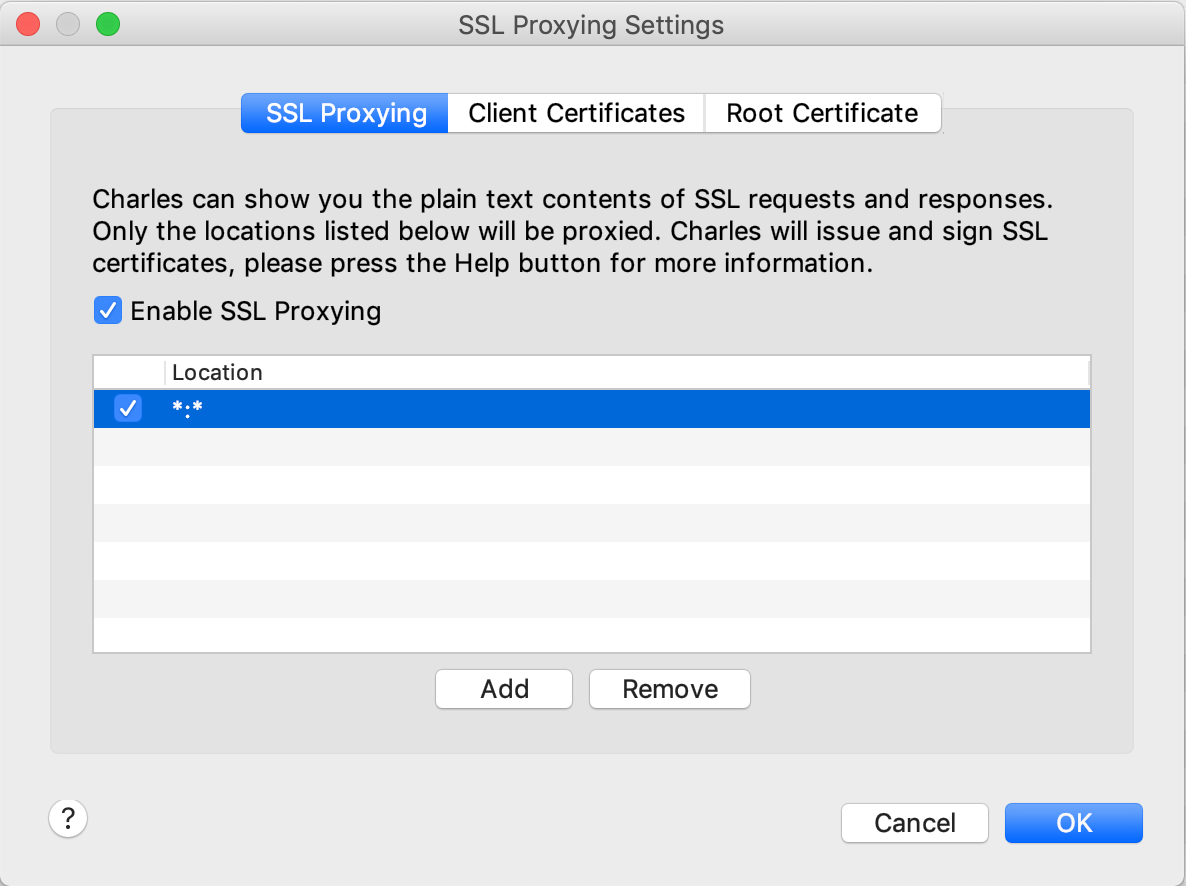
\includegraphics[width=0.8\textwidth]{img/charlessslsettings.png}
    \caption{Screenshot van de correcte SSL Proxying Settings binnen Charles}
    \label{fig:charlessslsettings}
\end{figure}

Dit is jammergenoeg nog niet het einde van het SSL-certificaat-verhaal. Apps die ontwikkeld zijn met Android 6.0 of lager als doelversie, zullen automatisch certificaten aanvaarden die door gebruikers geïnstalleerd zijn. Vanaf dat de applicatie gericht is op een hogere van Android, heeft de ontwikkelaar de mogelijkheid om 'SSL Certificate Pinning' toe te passen. Dit houdt in dat de ontwikkelaar, indien hij/zij dit wil, kan afdwingen dat er een bepaald certificaat wordt gebruikt wanneer er met zijn server gecommuniceerd wordt \autocite{wass_ssl-pinning}. Hier zal het Charles certificaat afgewezen worden, de aanvraag zal falen en de data die voortkomt uit het monitoren van de netwerkactiviteit is mogelijk niet meer volledig correct.

Er bestaan wel tools zoals 'frida' die tijdens het uitvoeren van een bepaalde applicatie het afgedwongen certificaat kunnen wijzigen, waardoor aanvragen wel doorkomen. Deze methoden vereisen echter root en zijn niet geschikt voor gebruik in dit experiment.

%TODO EMAIL DOUGLAS C SCHMIDT PLS ANTWOORD AUB PLS I NEED U

\section{Verloop experiment}
\label{sec:conditionsexperiment}
Binnen deze sectie zal worden besproken hoe het experiment precies zal verlopen en welke voorwaarden van toepassing zijn.

\subsection{Uitschrijven stappenplan per testgeval}
Per testgeval zal een stappenplan worden uitschreven dat in detail vermeld hoe de juiste situatie van het testgeval bereikt wordt. Indien hier moeilijkheden bij verlopen, dienen die ook opgenomen te worden.

\subsection{Meten van verzamelde data}
Bij alle testgevallen zullen Wi-Fi, bluetooth, en locatie ingeschakeld zijn. Dit wordt gedaan zodat er op elk moment genoeg data is die mogelijks naar Google kan worden verzonden. Wanneer de mogelijk te verzamelen data groter is, zorgt dit ook voor preciesere metingen van de werkelijk doorgestuurde data. Ook  testen we tot op welke mate we dataverzameling kunnen beperken sonder functionaliteit te beperken. Wanneer we deze verbindingsmethoden uitschakelen, wordt de functionaliteit van het apparaat beperkt. Het testapparaat zal via een 5 GHz Wi-Fi verbinding verbonden zijn met een beveiligd Wi-Fi netwerk. Mobiele data zal uitgeschakeld blijven, aangezien we via de gebruikte software hiervan de netwerkactiviteit niet kunnen monitoren.

Gedurende 1 uur zal de netwerkactiviteit van het apparaat gemonitord worden. Tijdens deze tijd zal het apparaat stilliggen en zal er ook geen interactie met het apparaat gebeuren. Het apparaat zal ook zodanig ingesteld zijn dat deze niet in slaapmodus valt, wat mogelijk de resultaten kan beïnvloeden. Er wordt niet gebruik gemaakt van modussen die de batterijduur zouden verlengen, en het apparaat zal tijdens het experiment aangesloten zijn aan zijn oplader. Voor elk testgeval zal een nieuw Google account gebruikt worden, indien vereist. Dit experiment kan meerdere keren uitgevoerd worden voor een betere benadering van realistische data.




